\section{Method}
\label{sec:method}

\subsection{Background for notation}
Given a video with RGB frames $\{\mathbf{I}^{\text{rgb}}_t\}_{t=1}^{T}$, our pipeline outputs a set of bird bounding boxes
$\mathcal{B}_t=\{b_t^n\}_{n=1}^{N_t}$ per frame and a set of tracks $\mathcal{T}_t=\{\tau_t^i\}_{i=1}^{M_t}$ over time.
We use pixel coordinates $\mathbf{x}=(x,y)^\top$.

\begin{figure*}[t]
  \centering
  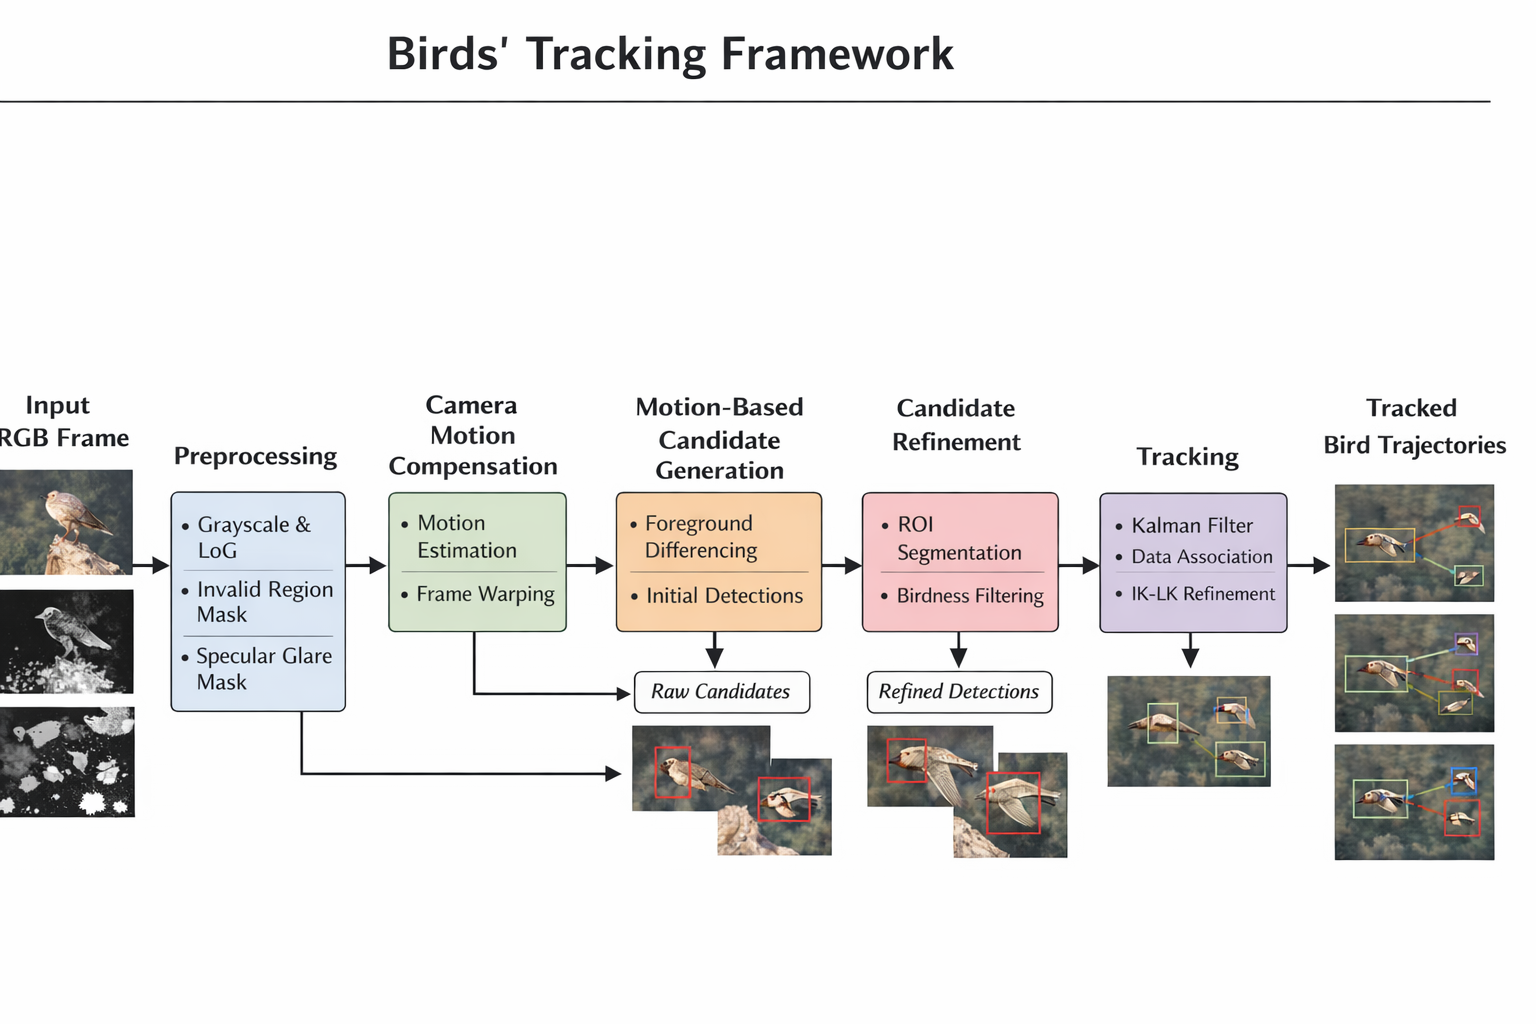
\includegraphics[width=0.45\textwidth]{pic_framework.png}
  \caption{Birds' Track Framework.}
  \label{fig:birds_framework}
\end{figure*}

\paragraph{Preprocessing outputs.}
From each frame we compute:
(1) a smoothed grayscale intensity image $I_t \in [0,255]^{H\times W}$,
(2) a Laplacian-of-Gaussian (LoG) feature map $L_t \in [0,255]^{H\times W}$,
(3) a hard valid mask $V_t \in \{0,255\}^{H\times W}$ (e.g., subtitles as invalid), and
(4) a soft specular/glare mask $S_t \in \{0,255\}^{H\times W}$ (glare-like regions as $0$).

\paragraph{Camera motion model.}
We estimate an affine warp $\mathbf{T}_t\in\mathbb{R}^{2\times 3}$ that aligns frame $(t\!-\!1)$ to $t$.
Let $\mathcal{W}(\mathbf{x};\mathbf{T}_t)$ denote the warped coordinate. The aligned previous feature is
\begin{equation}
\widehat{X}_{t-1\rightarrow t}(\mathbf{x}) = X_{t-1}\big(\mathcal{W}(\mathbf{x};\mathbf{T}_t)\big),
\end{equation}
where $X\in\{I,L\}$ depending on the stage.

\paragraph{Track state.}
Each track $\tau^i$ maintains a 2D constant-velocity state
\begin{equation}
\mathbf{s}^i_t = [c^i_{x,t},\,c^i_{y,t},\,v^i_{x,t},\,v^i_{y,t},\,w^i_t,\,h^i_t]^\top,
\end{equation}
with bounding box decoding
$b(\mathbf{s}^i_t)=\big(\lfloor c_x-\tfrac{w}{2}\rfloor,\ \lfloor c_y-\tfrac{h}{2}\rfloor,\ w,\ h\big)$.

\subsection{Preprocessing}
Bird flocks in the wild exhibit strong illumination changes and glare. We therefore compute both an intensity stream and a LoG stream.

\paragraph{Background smoothing.}
We first convert $\mathbf{I}^{\text{rgb}}_t$ to grayscale and apply edge-preserving smoothing to suppress high-frequency texture:
\begin{equation}
I_t = \texttt{Smooth}\big(\texttt{Gray}(\mathbf{I}^{\text{rgb}}_t)\big).
\end{equation}

\paragraph{LoG with local normalization.}
To be more robust to global brightening/darkening, we compute a LoG-like response and optionally normalize by local energy:
\begin{align}
\widetilde{I}_t &= G_{\sigma}\ast \texttt{Gray}(\mathbf{I}^{\text{rgb}}_t),\\
\Delta_t &= \left|\nabla^2 \widetilde{I}_t\right|,\\
L'_t &= \frac{\Delta_t}{G_{\sigma_e}\ast \Delta_t + \epsilon},\\
L_t &= \texttt{RobustRescale}(L'_t)\in[0,255].
\end{align}

\paragraph{Invalid region mask (subtitles).}
We build a hard mask $V_t$ by detecting subtitle-like components in a bottom ROI and marking them as invalid ($0$). The valid region remains $255$:
\begin{equation}
V_t(\mathbf{x})=
\begin{cases}
0, & \mathbf{x}\ \text{belongs to subtitle region},\\
255, & \text{otherwise}.
\end{cases}
\end{equation}

\paragraph{Specular/glare mask.}
We detect glare-like pixels (e.g., high $V$ with low $S$ in HSV and local contrast constraints) and output a soft mask $S_t$:
\begin{equation}
S_t(\mathbf{x})=
\begin{cases}
0, & \mathbf{x}\ \text{is glare-like},\\
255, & \text{otherwise}.
\end{cases}
\end{equation}
When the detected glare ratio is abnormally high, we safely bypass glare suppression by setting $S_t\equiv 255$.

\paragraph{Mask hole-filling for stable operators.}
To prevent strong false signals on subtitle boundaries, invalid regions can be filled by replacing them with a blurred version of the image:
\begin{equation}
I^{\text{fill}}_t(\mathbf{x})=
\begin{cases}
(G_{\sigma_f}\ast I_t)(\mathbf{x}), & V_t(\mathbf{x})=0,\\
I_t(\mathbf{x}), & V_t(\mathbf{x})>0.
\end{cases}
\end{equation}

\subsection{Camera Motion Compensation}
Even small camera motion can dominate frame differencing for tiny birds. We estimate $\mathbf{T}_t$ and warp the previous frame/feature accordingly.

\paragraph{Weighted phase correlation (Stage 1/2).}
We suppress invalid and glare-like regions by constructing a weight map $w(\mathbf{x})\in[0,1]$ from $V_t$ and $S_t$.
We apply weighted zero-mean normalization and estimate a translation $(\Delta x,\Delta y)$ using phase correlation.
We accept the estimate only if (i) the response is high, (ii) the shift magnitude is within a bound, and (iii) the alignment reduces a robust error metric:
\begin{equation}
\text{err}(A,B) = \texttt{median}\big(|A(\mathbf{x})-B(\mathbf{x})|\big)\ \text{over valid pixels.}
\end{equation}

\paragraph{ROI-consensus refinement (Stage 2).}
If global phase correlation is unreliable, we compute multiple translations on a set of ROIs (corners/strips). Each ROI measurement is weighted by
its phase-correlation response, valid fraction, and corner richness (Shi--Tomasi). We take a weighted median shift and apply MAD-based outlier rejection.

\paragraph{ECC fallback (Stage 3).}
When phase-correlation fails, we refine $\mathbf{T}_t$ using ECC alignment with increasing warp flexibility:
Euclidean $\rightarrow$ affine. We keep the warp only if it improves the robust error and clamp translation to a maximum magnitude.

\paragraph{Motion decision.}
We label camera motion as present if the maximum corner displacement induced by $\mathbf{T}_t$ exceeds a small threshold.

\subsection{Motion-Based Candidate Generation}
Given $I_t, L_t$ and aligned features $\widehat{I}_{t-1\rightarrow t}, \widehat{L}_{t-1\rightarrow t}$, we generate a foreground motion mask and convert it to candidate boxes.

\paragraph{Neutralize invalid regions.}
To ensure subtitle regions do not contaminate differences, we set the previous invalid pixels equal to current pixels so that the invalid-region diff becomes $0$.

\paragraph{Normalized intensity difference.}
We compute a normalized intensity difference map (robust to brightness scaling):
\begin{equation}
D^{\text{int}}_t(\mathbf{x})=\frac{\left|I_t(\mathbf{x})-\widehat{I}_{t-1\rightarrow t}(\mathbf{x})\right|}
{I_t(\mathbf{x})+\widehat{I}_{t-1\rightarrow t}(\mathbf{x})+\epsilon}.
\end{equation}

\paragraph{LoG difference and weighted fusion.}
If LoG features are available, we compute
\begin{equation}
D^{\text{log}}_t(\mathbf{x})=\left|L_t(\mathbf{x})-\widehat{L}_{t-1\rightarrow t}(\mathbf{x})\right|,
\end{equation}
and fuse the two streams in the difference domain:
\begin{equation}
D_t = (1-\lambda)\,\widetilde{D}^{\text{int}}_t + \lambda\,\widetilde{D}^{\text{log}}_t,\quad \lambda\in[0,1],
\end{equation}
where $\widetilde{D}$ denotes optional glare suppression (next).

\paragraph{Glare suppression on diff maps.}
Inside glare-like regions ($S_t(\mathbf{x})=0$), we down-weight the diff response:
\begin{equation}
\widetilde{D}_t(\mathbf{x})=
\begin{cases}
\alpha_{\text{spec}}\,D_t(\mathbf{x}), & S_t(\mathbf{x})=0\ \wedge\ V_t(\mathbf{x})>0,\\
D_t(\mathbf{x}), & \text{otherwise},
\end{cases}
\end{equation}
and bypass this step if glare occupies too large a fraction of the valid region.

\paragraph{Dual-threshold reconstruction.}
We compute a high threshold $\tau_h$ and low threshold $\tau_l$ from robust percentiles of $D_t$ in the valid region.
We form seed and candidate masks:
\begin{equation}
M_h=\mathbb{I}[D_t>\tau_h],\qquad M_l=\mathbb{I}[D_t>\tau_l],
\end{equation}
and iteratively reconstruct foreground by constrained dilation:
\begin{equation}
M^{(k+1)}=\big(\texttt{dilate}(M^{(k)})\big)\wedge M_l,\quad M^{(0)}=M_h,
\end{equation}
until convergence or a maximum number of iterations. The output motion mask is $M_t=M^{(K)}\wedge \mathbb{I}[V_t>0]$.

\paragraph{Morphology, components, and box post-processing.}
We apply resolution-scaled open/close and a light ``bridge'' operation to connect fragmented bird motion.
We extract connected components, filter by area/aspect ratio, and optionally split overly large components by erosion and re-growing.
Each component yields a padded bounding box with a score defined by the mean diff value inside the region.
Finally, we remove nested boxes using intersection-over-area (IoA) suppression and merge close boxes if they overlap (IoU) or their centers are near.

\subsection{Candidate Refinement}
The motion mask can still contain background fragments (waves, foliage). We refine each raw box using ROI-level instance separation and birdness constraints.

\paragraph{ROI foreground cleanup.}
For each raw box $b=(x,y,w,h)$, we crop the ROI from $M_t$ and apply open/close. If the number of foreground pixels is too small, we discard it.

\paragraph{Watershed-based splitting.}
Let $\text{fg}\in\{0,1\}^{h\times w}$ be the ROI foreground. We compute a distance transform:
\begin{equation}
\text{dist}=\texttt{DT}(\text{fg}),
\end{equation}
and build sure-foreground markers by thresholding:
\begin{equation}
\text{sure\_fg}=\mathbb{I}\left[\text{dist} > \rho\cdot \max(\text{dist})\right],\quad \rho\in(0,1).
\end{equation}
We then run watershed on the RGB ROI to separate instances and convert each instance into a bounding box.

\paragraph{Geometric and photometric constraints.}
We keep an instance box only if it satisfies:
(i) area bounds relative to the full image,
(ii) minimum side length,
(iii) aspect ratio bounds,
(iv) foreground occupancy inside the box (foreground ratio),
(v) instance fill ratio,
and (vi) a glare constraint (discard boxes mostly inside spec regions).
Per raw box, we keep the largest remaining instance to avoid duplicated boxes for one bird.

\subsection{Tracking}
We associate refined boxes across time and output stable tracklets. Our method uses: (i) a Kalman-like constant-velocity predictor,
(ii) gated association with a hybrid IoU-distance cost, (iii) track management, and (iv) Iterative Lucas--Kanade (IK-LK) refinement (as specified in the technical report).

\paragraph{Constant-velocity prediction and update.}
For each track $i$, we predict
\begin{equation}
\mathbf{c}^{i-}_t=\mathbf{c}^i_{t-1}+\mathbf{v}^i_{t-1},\qquad \mathbf{v}^{i-}_t=\mathbf{v}^i_{t-1},
\end{equation}
where $\mathbf{c}=(c_x,c_y)^\top$.
Given an associated detection with center $\mathbf{c}^{\text{det}}_t$, we update velocity by exponential smoothing:
\begin{equation}
\mathbf{v}^i_t = \beta\,\mathbf{v}^{i-}_t + (1-\beta)\big(\mathbf{c}^{\text{det}}_t-\mathbf{c}^{i-}_t\big),\quad \beta\in[0,1],
\end{equation}
and set $\mathbf{c}^i_t=\mathbf{c}^{\text{det}}_t$ while updating $(w,h)$ from the detection.

\paragraph{Gated association with hybrid cost.}
For a predicted track box $b^i$ and a detection box $b^j$, we define
\begin{equation}
\text{cost}(i,j)=w_{\text{iou}}\,(1-\text{IoU}(b^i,b^j)) + w_{\text{dist}}\,\frac{\|\mathbf{c}(b^i)-\mathbf{c}(b^j)\|_2}{\text{diag}(b^i)}.
\end{equation}
We only consider feasible pairs if they pass gates:
\begin{equation}
\text{IoU}(b^i,b^j)\ge \tau_{\text{iou}},\qquad
\|\mathbf{c}(b^i)-\mathbf{c}(b^j)\|_2 \le \gamma\cdot \text{diag}(b^i).
\end{equation}
We then solve assignment using a global greedy selection over all feasible pairs sorted by increasing cost
(optionally replaceable by Hungarian for exact bipartite matching).

\paragraph{Track management.}
Unmatched tracks increase a miss counter and are removed if $\text{miss}>\text{max\_age}$.
Unmatched detections spawn new tracks only if they are not too close to existing tracks (birth gate):
\begin{equation}
\max_i \text{IoU}(b^i,b^{\text{new}}) \le \tau_{\text{birth-iou}}
\quad\wedge\quad
\min_i \frac{\|\mathbf{c}(b^i)-\mathbf{c}(b^{\text{new}})\|_2}{\text{diag}(b^i)} \ge \tau_{\text{birth-dist}}.
\end{equation}
A track is reported as \emph{confirmed} only after reaching $\text{min\_hits}$ matches to suppress flickering false positives.

\paragraph{Iterative Lucas--Kanade Algorithm (general formulation, iterative version).}
To improve short-term localization and robustness to missed detections, we refine per-track displacement between consecutive frames using IK-LK.
Let $I(\mathbf{x})$ be the template patch from the previous frame (e.g., around the predicted track location),
and let $J(\mathbf{x})$ be the current-frame patch. We seek a translation $\mathbf{d}$ such that
$I(\mathbf{x}) \approx J(\mathbf{x}+\mathbf{d})$.
We initialize $\bar{\nu}_0$ by the motion-model prediction (or zero), and iterate:

\begin{align}
\bar{\eta}_k &= G^{-1}\,b_k,\\
b_k &= \sum_{\mathbf{x}}\begin{bmatrix}
\delta I_k(\mathbf{x})\,I_x(\mathbf{x})\\
\delta I_k(\mathbf{x})\,I_y(\mathbf{x})
\end{bmatrix},\qquad
\delta I_k(\mathbf{x}) = I(\mathbf{x}) - J_k(\mathbf{x}),\\
J_k(\mathbf{x}) &= J(\mathbf{x}+\bar{\nu}_{k-1}),
\end{align}
where $I_x,I_y$ are spatial gradients of the template (computed once), and
\begin{equation}
G=\sum_{\mathbf{x}}
\begin{bmatrix}
I_x(\mathbf{x})^2 & I_x(\mathbf{x})I_y(\mathbf{x})\\
I_x(\mathbf{x})I_y(\mathbf{x}) & I_y(\mathbf{x})^2
\end{bmatrix}
\end{equation}
is constant across iterations. After computing $\bar{\eta}_k$, we update the displacement hypothesis:
\begin{equation}
\bar{\nu}_k=\bar{\nu}_{k-1}+\bar{\eta}_k.
\end{equation}
We iterate until $\|\bar{\eta}_k\|_2$ is below a threshold or a fixed number of iterations is reached. The final displacement is
\begin{equation}
\bar{\nu}=\mathbf{d}=\sum_{k=1}^{K}\bar{\eta}_k=\bar{\nu}_K.
\end{equation}

\paragraph{Using IK-LK in tracking.}
For each active track, we run IK-LK on an intensity patch (optionally after camera-motion compensation) and refine the predicted center:
$\mathbf{c}^{i-}_t \leftarrow \mathbf{c}^{i-}_t + \mathbf{d}$.
This refined prediction is then used for association (or, if no detection matches, for short-term propagation within $\text{max\_age}$).